\documentclass[10pt, a4paper]{article}
\usepackage[paper=a4paper, left=1.5cm, right=1.5cm, bottom=1.5cm, top=2cm]{geometry}
\usepackage[utf8]{inputenc}
\usepackage[T1]{fontenc}
\usepackage[spanish]{babel}
\usepackage{indentfirst}
\usepackage{fancyhdr}
\usepackage{lastpage}
\usepackage{calc}
\usepackage{caratula}
\usepackage{marvosym} % para \Faxmachine !
\usepackage{graphicx}
\usepackage{float}
% \PassOptionsToPackage{noend}{algpseudocode}% comment out if want end's to show
\usepackage{algpseudocode}
\usepackage{algorithm}
\usepackage{multicol}
\usepackage[hidelinks]{hyperref}
\graphicspath{{imagenes/}}
%\sloppy
\parskip=5pt % 10pt es el tamano de fuente

\usepackage{stringenc}
\usepackage{pdfescape}
\usepackage{color}
\definecolor{red}{RGB}{255,0,0}
\definecolor{blue}{RGB}{0,0,255}
\usepackage{amsmath}
\usepackage[makeroom]{cancel}
\usepackage{wrapfig}
\usepackage[font=small,labelfont=bf]{caption}
\usepackage{amssymb}% http://ctan.org/pkg/amssymb
\usepackage{pifont}% http://ctan.org/pkg/pifont
\newcommand{\cmark}{\ding{51}}%
\newcommand{\xmark}{\ding{55}}%

%% -------------------------
\errorcontextlines\maxdimen

% begin vertical rule patch for algorithmicx (http://tex.stackexchange.com/questions/144840/vertical-loop-block-lines-in-algorithmicx-with-noend-option)
\makeatletter
% start with some helper code
% This is the vertical rule that is inserted
    \newcommand*{\algrule}[1][\algorithmicindent]{\makebox[#1][l]{\hspace*{.5em}\thealgruleextra\vrule height \thealgruleheight depth \thealgruledepth}}%
% its height and depth need to be adjustable
\newcommand*{\thealgruleextra}{}
\newcommand*{\thealgruleheight}{.75\baselineskip}
\newcommand*{\thealgruledepth}{.25\baselineskip}

\newcount\ALG@printindent@tempcnta
\def\ALG@printindent{%
    \ifnum \theALG@nested>0% is there anything to print
        \ifx\ALG@text\ALG@x@notext% is this an end group without any text?
            % do nothing
        \else
            \unskip
            \addvspace{-1pt}% FUDGE to make the rules line up
            % draw a rule for each indent level
            \ALG@printindent@tempcnta=1
            \loop
                \algrule[\csname ALG@ind@\the\ALG@printindent@tempcnta\endcsname]%
                \advance \ALG@printindent@tempcnta 1
            \ifnum \ALG@printindent@tempcnta<\numexpr\theALG@nested+1\relax% can't do <=, so add one to RHS and use < instead
            \repeat
        \fi
    \fi
    }%
\usepackage{etoolbox}
% the following line injects our new indent handling code in place of the default spacing
\patchcmd{\ALG@doentity}{\noindent\hskip\ALG@tlm}{\ALG@printindent}{}{\errmessage{failed to patch}}
\makeatother

% the required height and depth are set by measuring the content to be shown
% this means that the content is processed twice
\newbox\statebox
\newcommand{\myState}[1]{%
    \setbox\statebox=\vbox{#1}%
    \edef\thealgruleheight{\dimexpr \the\ht\statebox+1pt\relax}%
    \edef\thealgruledepth{\dimexpr \the\dp\statebox+1pt\relax}%
    \ifdim\thealgruleheight<.75\baselineskip
        \def\thealgruleheight{\dimexpr .75\baselineskip+1pt\relax}%
    \fi
    \ifdim\thealgruledepth<.25\baselineskip
        \def\thealgruledepth{\dimexpr .25\baselineskip+1pt\relax}%
    \fi
    %\showboxdepth=100
    %\showboxbreadth=100
    %\showbox\statebox
    \State #1%
    %\State \usebox\statebox
    %\State \unvbox\statebox
    %reset in case the next command is not wrapped in \myState
    \def\thealgruleheight{\dimexpr .75\baselineskip+1pt\relax}%
    \def\thealgruledepth{\dimexpr .25\baselineskip+1pt\relax}%
}
% end vertical rule patch for algorithmicx
%%--------------------------



\begin{document}
\title{TDC - TP2}
\materia{Teoría de las Comunicaciones}
\submateria{Segundo cuatrimestre 2017}
\titulo{Grupo 6}
\begin{center}
    
\includegraphics[width=0.7\textwidth]{caratula.jpg}
\end{center}
\subtitulo{TP2}
\integrante{Alejandro Ferrante}{371/09}{matapalabras@hotmail.com}
\integrante{Gonzalo Guillamon}{97/12}{gonzaguillamon@gmail.com}
\integrante{Malena Ivnisky}{421/12}{malenaivnisky@gmail.com}

\maketitle

% \newpage\null\thispagestyle{empty}

\newpage
\thispagestyle{empty}
\setcounter{tocdepth}{3}
\tableofcontents

% \newpage\null\thispagestyle{empty}

\newpage
\setcounter{page}{1}


%\includegraphics[width=\textwidth]{cookies}  ejemplo para incluir imagenes

\section{Resumen}
\section{Introducción}

El objetivo de este trabajo práctico es analizar distintas capturas de red usando las herramientas vistas en la materia.


\section{Implementación}
La herramienta se encuentra implementada en el archivo \texttt{traceroute.py}. Toma como parámetros la dirección a envíar los paquetes, el tamaño de las ráfagas de paquetes (\texttt{burst\_size}) y el máximo TTL.

Para cada TTL entre 1 y el máximo se envían \texttt{burst\_size} paquetes con el TTL adecuado y se reciben las respuestas, usando la función \texttt{sr()} de \texttt{scapy}. Si se recibe un echo reply, se dejan de mandar ráfagas.

A partir de los paquetes recibidos como respuesta de un TTL se obtiene una IP (la más común de entre los hosts que respondieron) y un RTT (el promedio de RTT para la IP elegida). Si no se recibe ninguna respuesta, ambos son nulos. Elegimos promediar sólo los RTT de los saltos con la IP elegida y no todos porque esto es más consistente con la elección.

Una vez procesados los envíos, empieza el análisis para predecir los saltos intercontinentales. Aplicamos el método de Cimbala para obtener los outliers, que serán los saltos intercontinentales predichos. Los datos a analizar son las diferencias de RTT en cada salto con el salto anterior no nulo. 

Los saltos con menor RTT que el inmediatamente anterior tienen una diferencia negativa, y decidimos ignorarlos en el análisis ya que no representan magnitudes reales.

%% podemos mandarle el pseudocodigo de cimbala o no ... no se P:

\section{Ruta 1: Universidad de Tokyo}

Ejecutamos la herramienta usando la dirección \texttt{www.u-tokyo.ac.jp}, con ráfagas de 100 paquetes y TTL máximo igual a 30. Los resultados obtenidos se muestran en las figuras \ref{tabla1} y \ref{mapa1}. Las ubicaciones indicadas fueron obtenidas usando una página de geolocalización de IP \cite{ip2location}.

\subsection{Análisis de la ruta obtenida}
Observamos que la ruta parte de Buenoa Aires como corresponde. Luego de no obtener respuesta en varios saltos, encontramos una IP supuestamente localizada en Italia. En el salto siguiente la IP se encuentra en Brasil.

Esto nos hizo sospechar acerca de la correctitud de esta ruta, ya que existen caminos directos entre Argentina y Brasil; no hay necesidad de pasar por Italia. Esto se puede ver en un mapa de cables submarinos \cite{cables}.

Como vimos que varias páginas de geolocalización de IP daban resultados distintos para la misma IP, usando una página que da resultados de fuentes distintas \cite{iplocation} comparamos resultados para la IP \texttt{195.22.219.3}. Obtuvimos como resultado que casi todas las fuentes devuelven una ubicación en Italia, mientras que una devuelve la ciudad de Fortaleza, en Brasil. Observamos que el cable submarino Altantis-2 conecta entre otras ciudades Las Toninas con Fortaleza \cite{atlantis2}. Además, figura como uno de los dueños del cable la empresa Telecom Italia Sparkle, que figura como ISP en varias búsquedas que ubican esta IP en Italia. Por esto creemos que la verdadera ruta va directamente hacia Fortaleza usando el cable Atlantis-2, ya que los métodos de geolocalización de IPs no son muy confiables \cite{accuracy}, y podría ocurrir que la ubicación de una IP situada físicamente en Brasil pero vinculada a una ISP italiana sea medida incorrectamente.

Luego la ruta sigue por San Pablo, y luego salta hasta Nueva York. En este caso mirando el mapa \cite{cables} vemos que se usa el cable Seabras-1, que une estas dos ciudades \cite{seabras1}.

Siguiendo por Estados Unidos, la ruta pasa por Seattle y salta hasta Osaka, en Japón. Esto es posible si se usa el cable Pacific Crossing-1, que entre otras ciudades une Shima, Japón (cercana a Osaka) con la zona de Seattle.

Finalmente se llega al destino en Tokyo.

\subsection{Análisis de las predicciones de salto intercontinental}




\begin{figure}[H]
\centering
\begin{tabular}{l | l | l | l | l}
Hop & RTT & IP & Ubicación & Predicción de SI & ¿correcto?\\
1 & 0.0200 & 192.168.0.1 & Buenos Aires, Argentina & true\\
2 & null & null & null & null\\
3 & null & null & null & null\\
4 & null & null & null & null\\
5 & null & null & null & null\\
6 & 0.0742 & \texttt{200.89.161.85} & Buenos Aires, Argentina & false\\
7 & 0.0369 & \texttt{200.89.165.197} & Buenos Aires, Argentina & true\\
8 & 0.0434 & \texttt{200.89.165.222} & Buenos Aires, Argentina & true\\
9 & 0.0219 & \texttt{185.70.203.32} & Buenos Aires, Argentina & true\\
10 & 0.0604 & \texttt{195.22.219.3} & Lombardia, Italia & true\\
11 & 0.1129 & \texttt{149.3.181.65} & San Pablo, Brasil & false\\
12 & 0.1700 & \texttt{129.250.2.227} & Nueva York, EEUU & true\\
13 & 0.2852 & \texttt{129.250.4.13} & Seattle, EEUU & true\\
14 & 0.4943 & \texttt{129.250.2.54} & Seattle, EEUU & true\\
15 & 0.4242 & \texttt{129.250.3.61} & Osaka, Japón & true\\
16 & 0.9055 & \texttt{129.250.5.41} & Osaka, Japón & true\\
17 & 0.6164 & \texttt{129.250.3.106} & Osaka, Japón & true\\
18 & 0.3777 & \texttt{61.200.80.218} & Osaka, Japón & true\\
19 & null & null & null & null\\
20 & null & null & null & null\\
21 & null & null & null & null\\
22 & 0.3522 & \texttt{154.34.240.254} & Tokyo, Japón & true\\
23 & 0.4735 & \texttt{210.152.135.178} & Tokyo, Japón & true\\
\end{tabular}
\caption{Tabla de resultados para la Universidad de Tokyo.}
\label{tabla1}
\end{figure}

\begin{figure}[H]
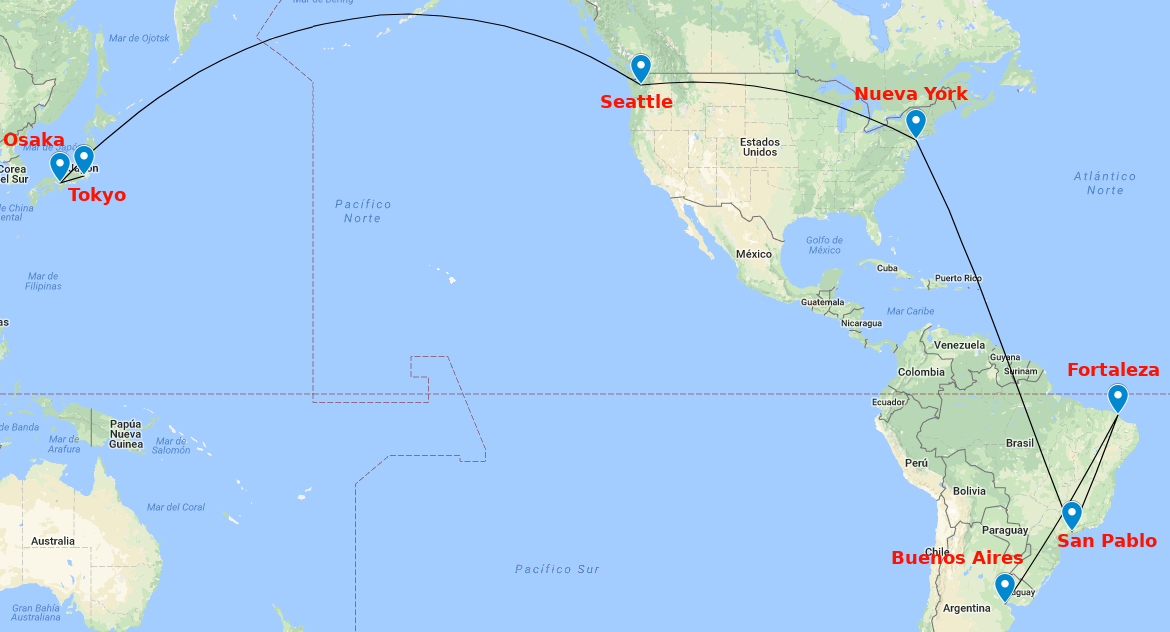
\includegraphics[width=\textwidth]{tokyo.png}
\caption{Mapa de resultados para la Universidad de Tokyo.}
\label{mapa1}
\end{figure}
\section{Ruta 2: Universidad de Ghana}

Ejecutamos la herramienta usando la dirección \texttt{www.ug.edu.gh}, y al igual que en el caso anterior con ráfagas de 100 paquetes y TTL máximo 30.

Realizamos un gráfico de la ruta obtenida usando una página de geolocalización por IP \cite{ip2location}, que se encuentra en la figura \ref{mapa2}.

\subsection{Análisis de la ruta obtenida}

La ruta parte de Buenos Aires, que es consistente ya que los paquetes fueron enviados desde ahí. Luego de no obtener respuesta en varios saltos, la siguiente respuesta sigue en Buenos Aires.

La ruta sigue en Estados Unidos, es posible que se utilice esta ruta a pesar de haber una más corta (según el mapa de cables subacuáticos \cite{cables}) porque al ser más utilizadas las comunicaciones entre Argentina y América del Norte (particularmente Estados Unidos) que con África, es posible que los paquetes vayan más rápido por esa ruta.

Luego hace un salto a Londres, que sería el segundo salto intercontinental. Siguiente, hace un salto a Singapur, que podría pensarse que se trata de un error de geolocalización. Sin embargo, el RTT es consistente con un envío por una ruta muy larga. De todas formas buscamos otras fuentes y vimos que la IP \texttt{195.219.195.42} podría estar ubicada en Inglaterra.

Luego los paquetes realizan varios saltos en Ghana hasta llegar a destino. 

Los saltos Buenos Aires-Ashburn, Ashburn-Londres y Singapur-Ghana son detectados correctamente. A la vez, hay muchos falsos positivos, en el caso del salto Londres-Singapur es entendible porque es un salto con un RTT muy alto, en los otros casos, pensamos que podría deberse a la aparición de RTTs con diferencia negativa con el salto anterior, que hacen que la detección de outliers sea peor.

\subsection{Análisis de las predicciones de salto intercontinental}

Calculamos las siguientes métricas de acuerdo a lo observado en la tabla \ref{tabla2}:

\begin{itemize}
	\item Porcentaje de saltos que no responden: 0\%
	\item Largo de la ruta de saltos que responden: 19 saltos 
	\item Cantidad de enlaces intercontinentales (separando América del Sur/Norte): 4
	\item Cantidad de outliers: 3
	\item Falsos positivos: 1
	\item Falsos negativos: 2
\end{itemize}

\begin{figure}[H]
\centering
\begin{tabular}{l | l | l | l | c | c}
Hop & RTT & IP & Ubicación & Predicción de SI & ¿correcto?\\
\hline
1 & 0.0021 & \texttt{192.168.10.1} & Buenos Aires, Argentina & false & \cmark\\
2 & 0.0060 & \texttt{192.168.0.1} & Buenos Aires, Argentina & false & \cmark\\
3 & 0.0167 & \texttt{10.31.0.1} & Buenos Aires, Argentina & false & \cmark\\
4 & 0.0141 & \texttt{10.242.2.133} & Buenos Aires, Argentina & false & \cmark\\
5 & 0.0133 & \texttt{195.22.220.33} & Buenos Aires, Argentina & false & \cmark\\
6 & 0.0147 & \texttt{195.22.220.32} & Buenos Aires, Argentina & false & \cmark\\
7 & 0.1584 & \texttt{195.22.199.191} & Ashburn, EEUU & true & \cmark\\
8 & 0.1714 & \texttt{216.6.87.202} & Ashburn, EEUU & false & \cmark\\
9 & 0.2308 & \texttt{216.6.87.138} & Newark, EEUU & true & \xmark\\
10 & 0.2228 & \texttt{216.6.57.1} & Newark, EEUU & false & \cmark\\
11 & 0.2224 & \texttt{80.231.130.33} & Londres, Inglaterra & false & \xmark\\
12 & 0.2251 & \texttt{80.231.130.130} & Londres, Inglaterra & false & \cmark\\
13 & 0.2218 & \texttt{80.231.76.121} & Londres, Inglaterra & false & \cmark\\
14 & 0.5116 & \texttt{195.219.195.42} & Singapur/Londres & true & \cmark\\
15 & 0.3219 & \texttt{41.204.60.149} & Kumasi, Ghana & false & \xmark\\
16 & 0.3336 & \texttt{41.204.60.150} & Kumasi, Ghana & false & \cmark\\
17 & 0.3298 & \texttt{197.255.127.6} & Accra, Ghana & false & \cmark\\
18 & 0.3453 & \texttt{197.255.127.35} & Accra, Ghana & false & \cmark\\
19 & 0.3393 & \texttt{197.255.125.213} & Accra, Ghana & false & \cmark\\
\end{tabular}
\caption{Tabla de resultados para la Universidad de Ghana.}
\label{tabla2}
\end{figure}

\begin{figure}[H]
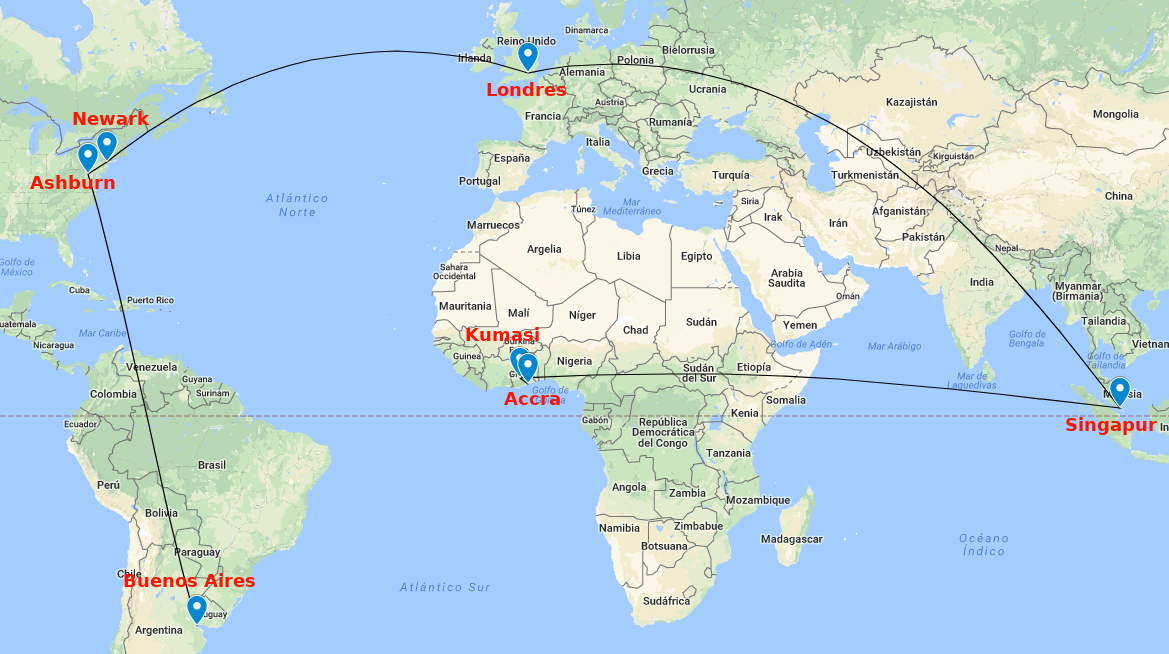
\includegraphics[width=\textwidth]{ghana.png}
\caption{Mapa de resultados para la Universidad de Ghana.}
\label{mapa2}
\end{figure}

En la figura \ref{diff1} se puede ver que la mayor diferencia se da en el salto 15, esto tiene sentido porque es el salto que va a Singapur. Aunque el siguiente salto es un salto con menor RTT, por lo que la herramienta no siempre debe estar tomando este salto. El resto de los puntos no muestran una tendencia definida (ni creciente ni decreciente).


\begin{figure}[H]
\centering
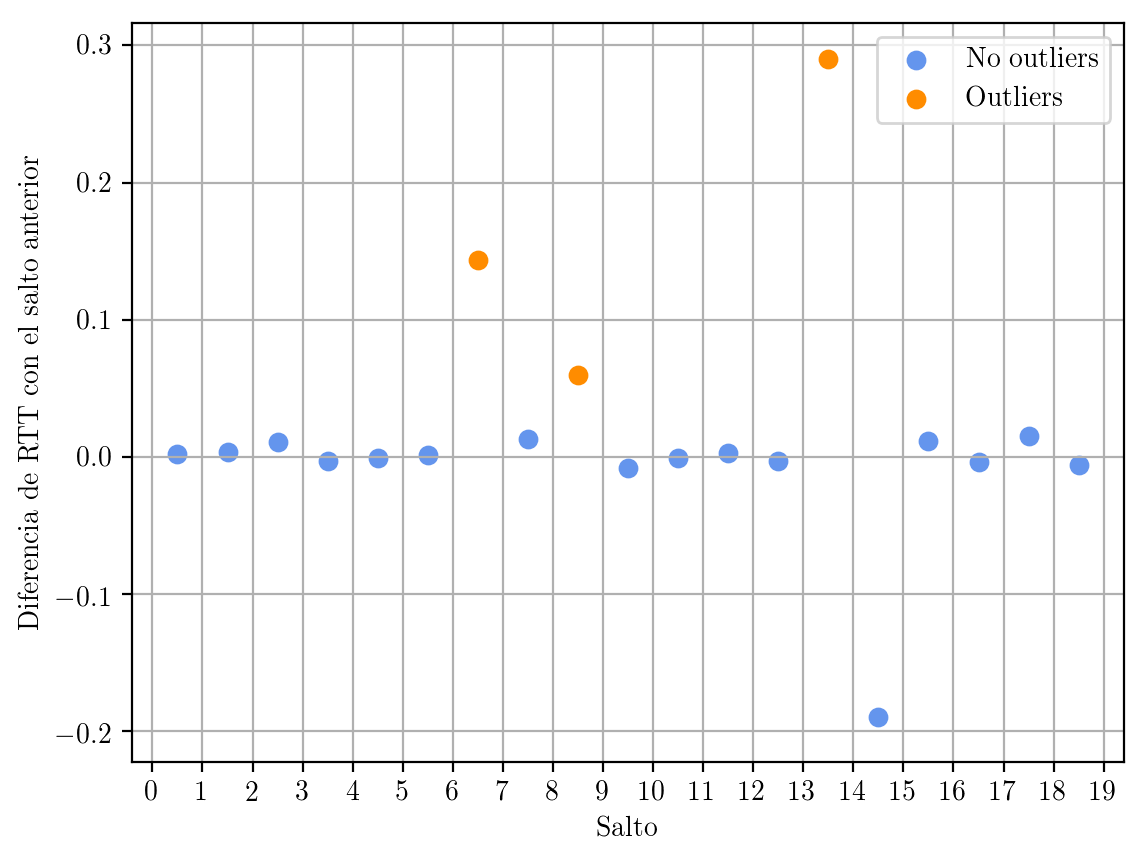
\includegraphics[width=0.6\textwidth]{ghana1.png}
\caption{Gráfico de diferencias de RTT en función de cada salto.}
\label{diff2}
\end{figure}

De la figura \ref{sdev2} vemos que también hay varios puntos están muy dispersos y por eso este experimento también devolvió muchos outliers como resultado.

\begin{figure}[H]
\centering
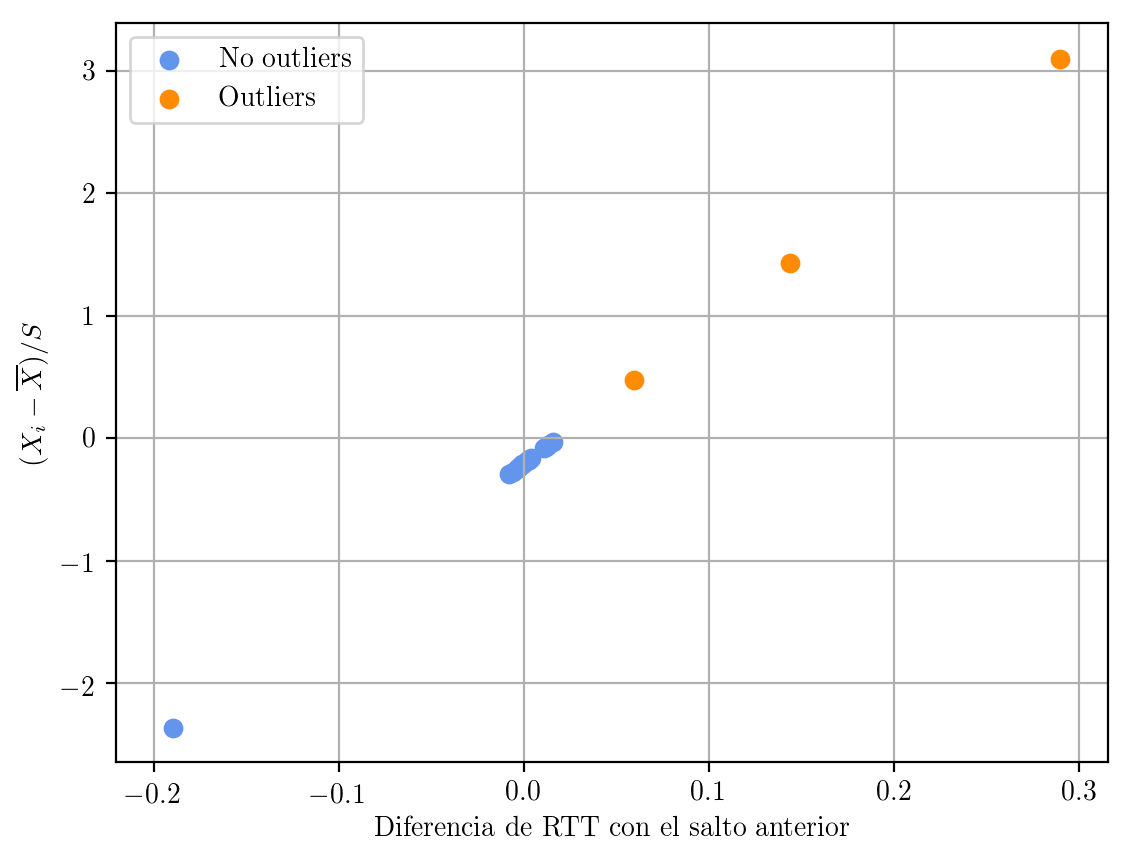
\includegraphics[width=0.6\textwidth]{ghana2.png}
\caption{Gráfico de $\frac{X_i - \bar{X}}{S}$ en función de las diferencias de RTT.}
\label{sdev2}
\end{figure}
\section{Ruta 3: Universidad de Ljubljana}

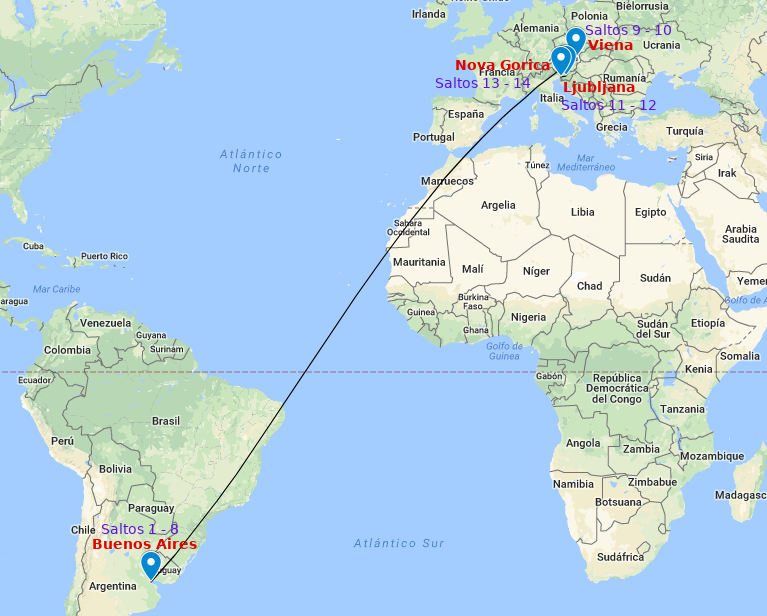
\includegraphics[width=\textwidth]{ljubljana.png}
\section{Conclusiones}

No vimos falsos negativos. En general hay outliers de más, no de menos. 

Este método no es muy efectivo porque las velocidades de internet en cada país no son las mismas, y eso no es tenido en cuenta.

Además, el hecho de que en cada envío los paquetes puedan tomar una ruta diferente hace que los experimentos devuelvan resultados con muchos outliers y datos inconsistentes.

Por otra parte, el analisis de las IPs visitadas era razonable, aunque el camino elegido no siempre fuera el más ``intuitivo''. Sin embargo, varios de los resultados que obtuvimos nos llevan a la conclusión de que tampoco son datos certeros.
\begin{thebibliography}{99}

\bibitem{ip2location}
  \texttt{https://www.ip2location.com/}

\bibitem{cables}
	\texttt{https://www.submarinecablemap.com/}

\bibitem{iplocation}
	\texttt{https://www.iplocation.net/}

\bibitem{atlantis2}
	\texttt{https://en.wikipedia.org/wiki/Atlantis-2}

\bibitem{accuracy}
	\texttt{https://www.iplocation.net/geolocation-accuracy}

\bibitem{seabras1}
	\texttt{https://en.wikipedia.org/wiki/Seaborn\_Networks}

\bibitem{pc1}
	\texttt{https://en.wikipedia.org/wiki/PC-1}

\bibitem{seamewe}
	\texttt{https://en.wikipedia.org/wiki/SEA-ME-WE\_3}

\bibitem{wacs}
	\texttt{https://en.wikipedia.org/wiki/WACS\_(cable\_system)}

\bibitem{glo1}
	\texttt{https://en.wikipedia.org/wiki/GLO-1}

\end{thebibliography}

\end{document}
